This appendix presents \emph{Pachelbel's Canon}. First only the melodic part, next the accompaniment
part and finally the whole score.

\section{Melody}
\label{sec:pcanon_melody}

This appendix presents \emph{Pachelbel's Canon}'s melodic part.\\

\lstinputlisting[caption={pachelbel\_canon\_melody.abc},captionpos=t,abovecaptionskip=-\medskipamount]{misc/pach_melody.tex}

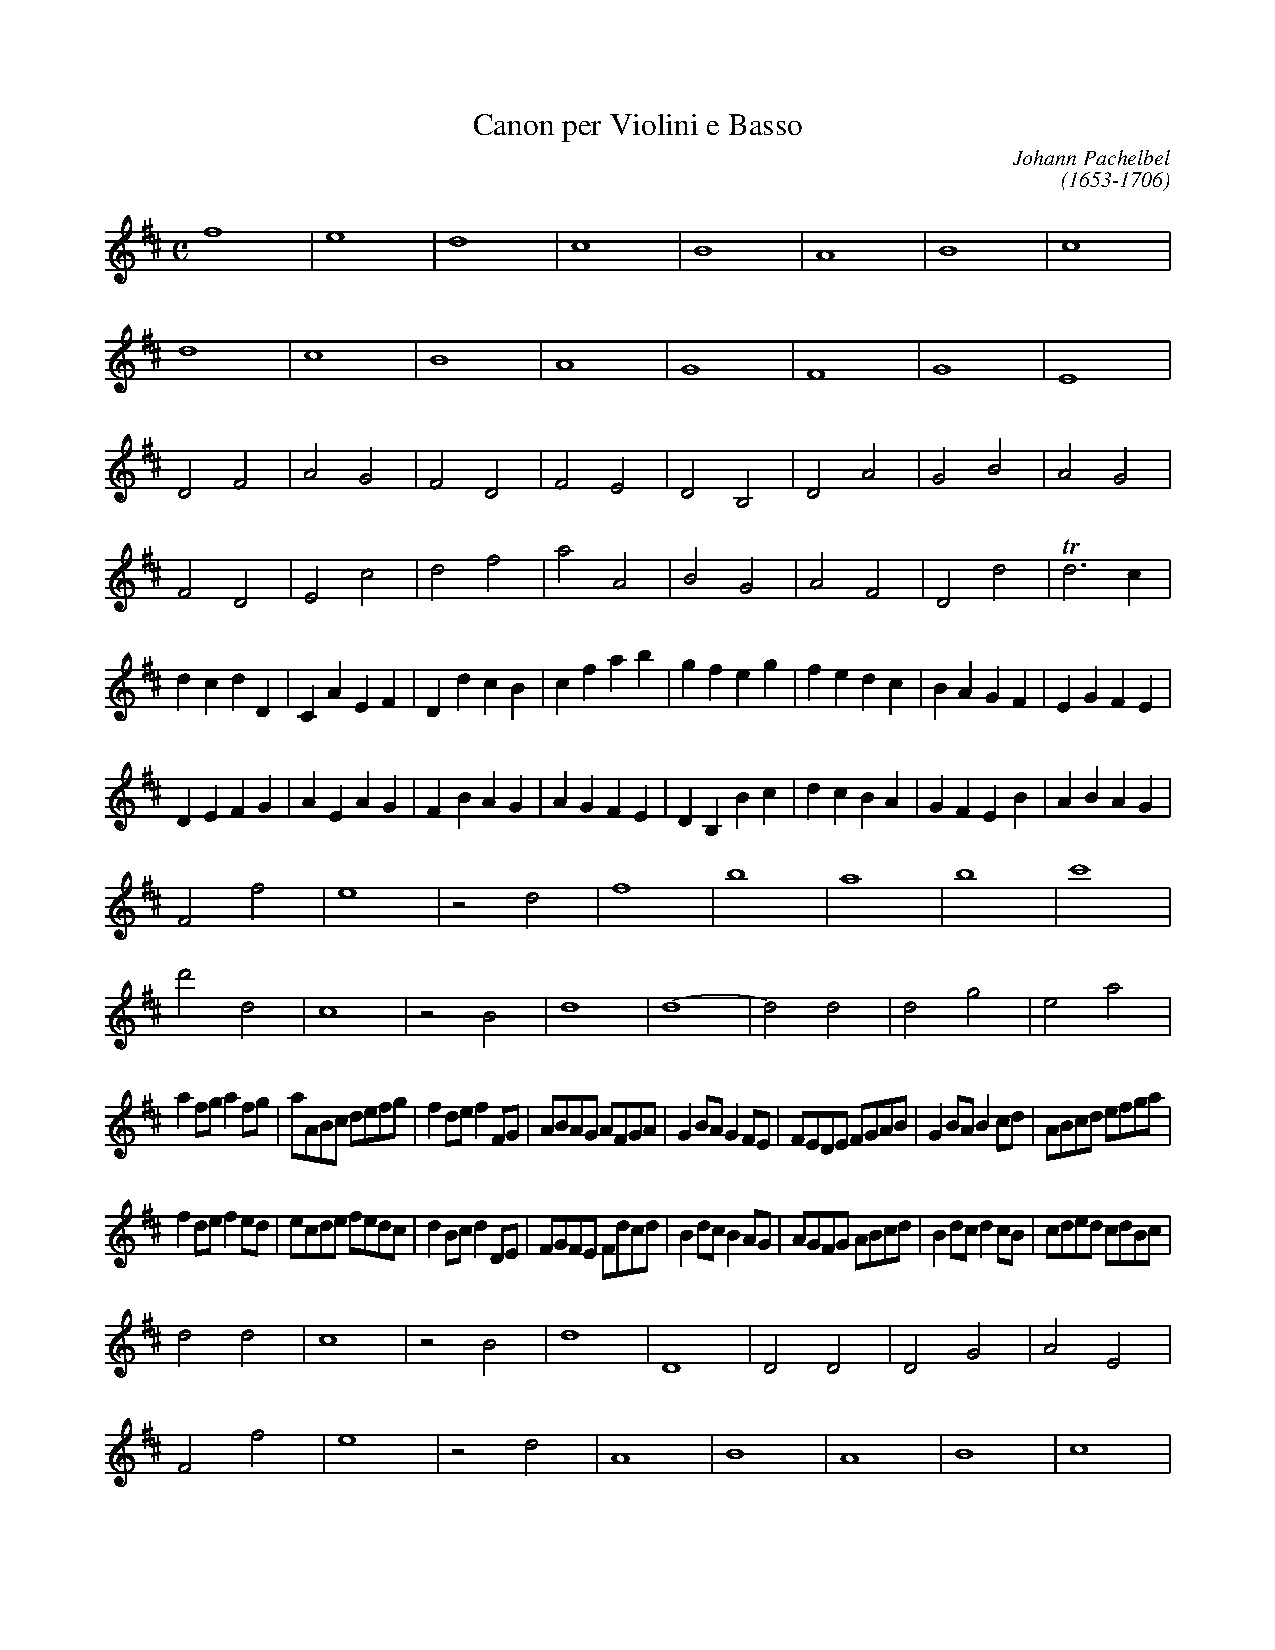
\includepdf[pages={1,2}]{img/pach_melody.pdf}

\section{Accompaniment}
\label{sec:pcanon_accomp}

This appendix presents \emph{Pachelbel's Canon}'s accompaniment part.\\

\lstinputlisting[caption={pachelbel\_canon\_accompaniment.abc},captionpos=t,abovecaptionskip=-\medskipamount]{misc/pach_accomp.tex}

\begin{figure}[H]
  \begin{center}
    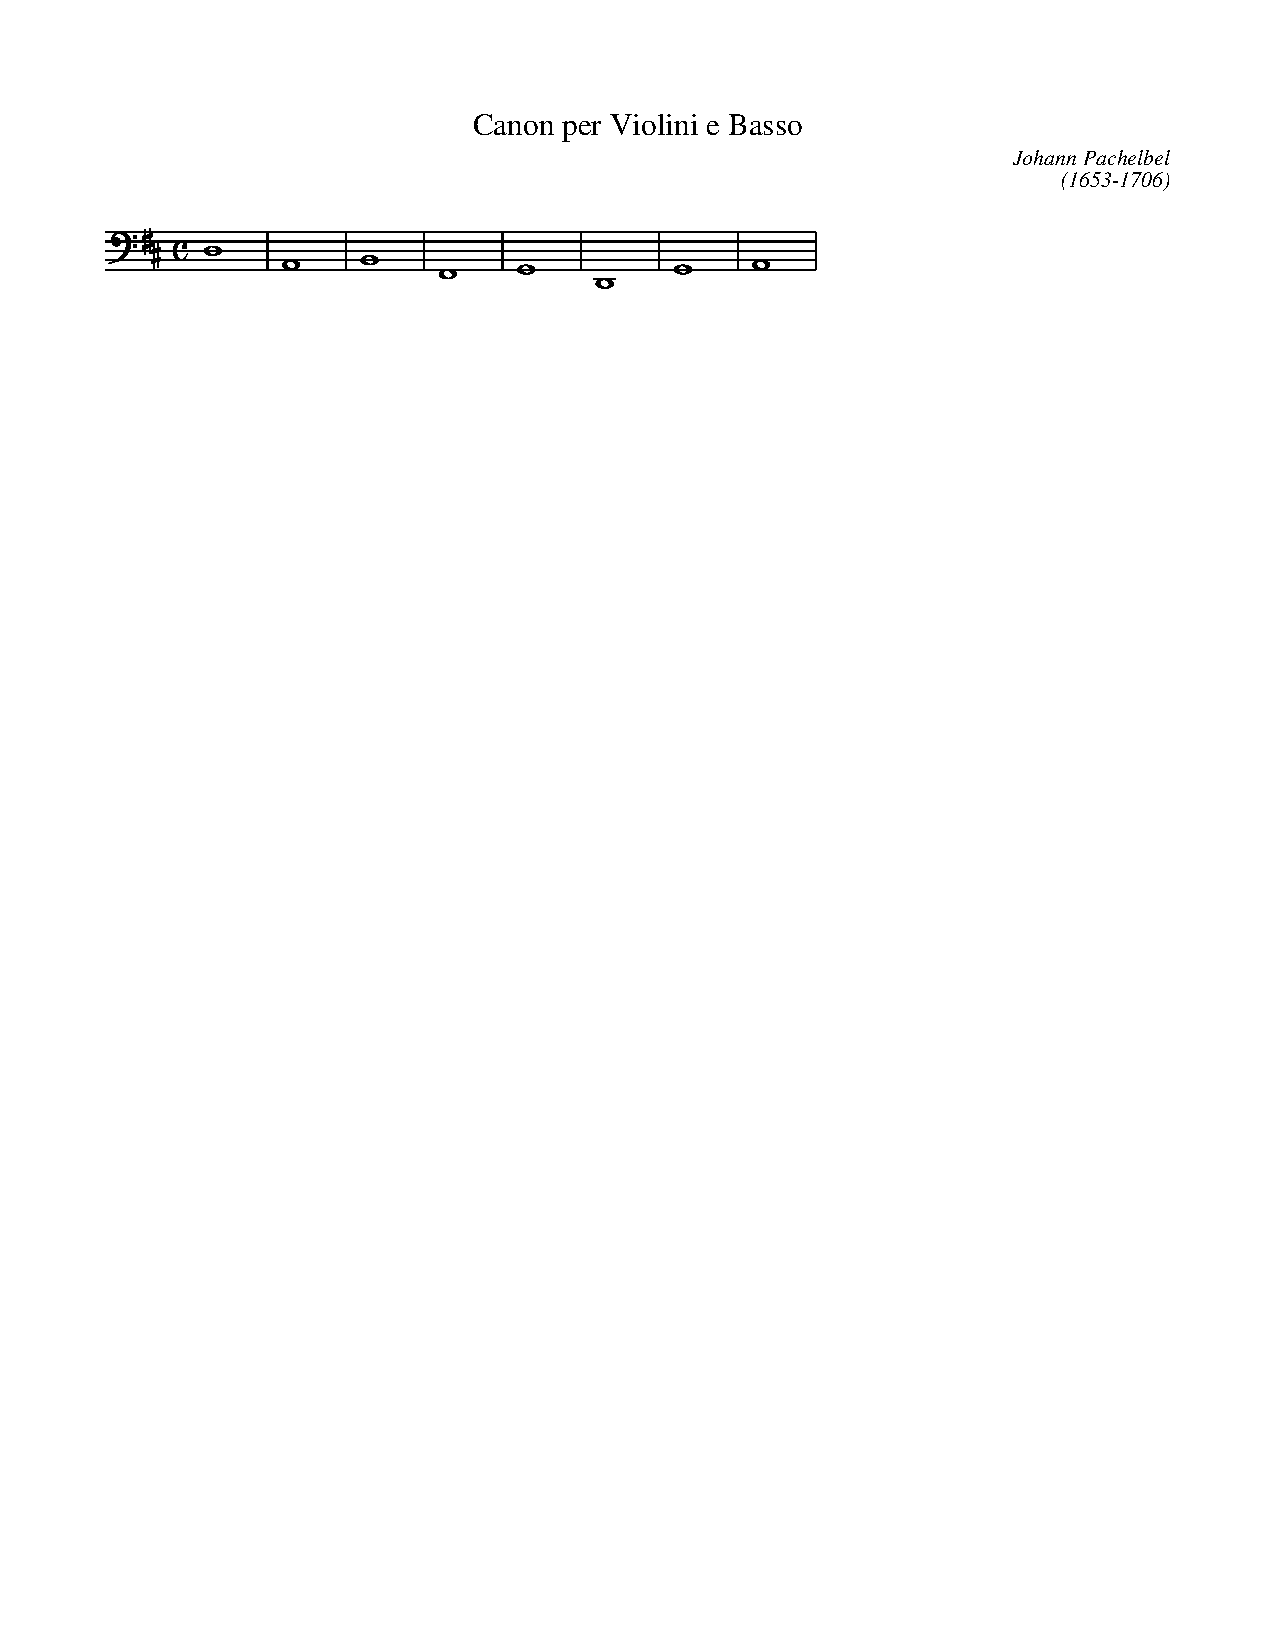
\includegraphics[width=1\textwidth, clip=true, trim = 17mm 230mm 17mm 19mm]{img/pach_accomp.pdf}
    \caption{Pachelbel's Canon accompaniment}
  \end{center}
\end{figure}

\section{Output generated by canon\_abc}
\label{sec:pcanon}

This appendix presents \emph{Pachelbel's Canon}'s whole score.\\

\lstinputlisting[caption={pachelbel\_canon.abc},captionpos=t,abovecaptionskip=-\medskipamount]{misc/pach_canon.tex}

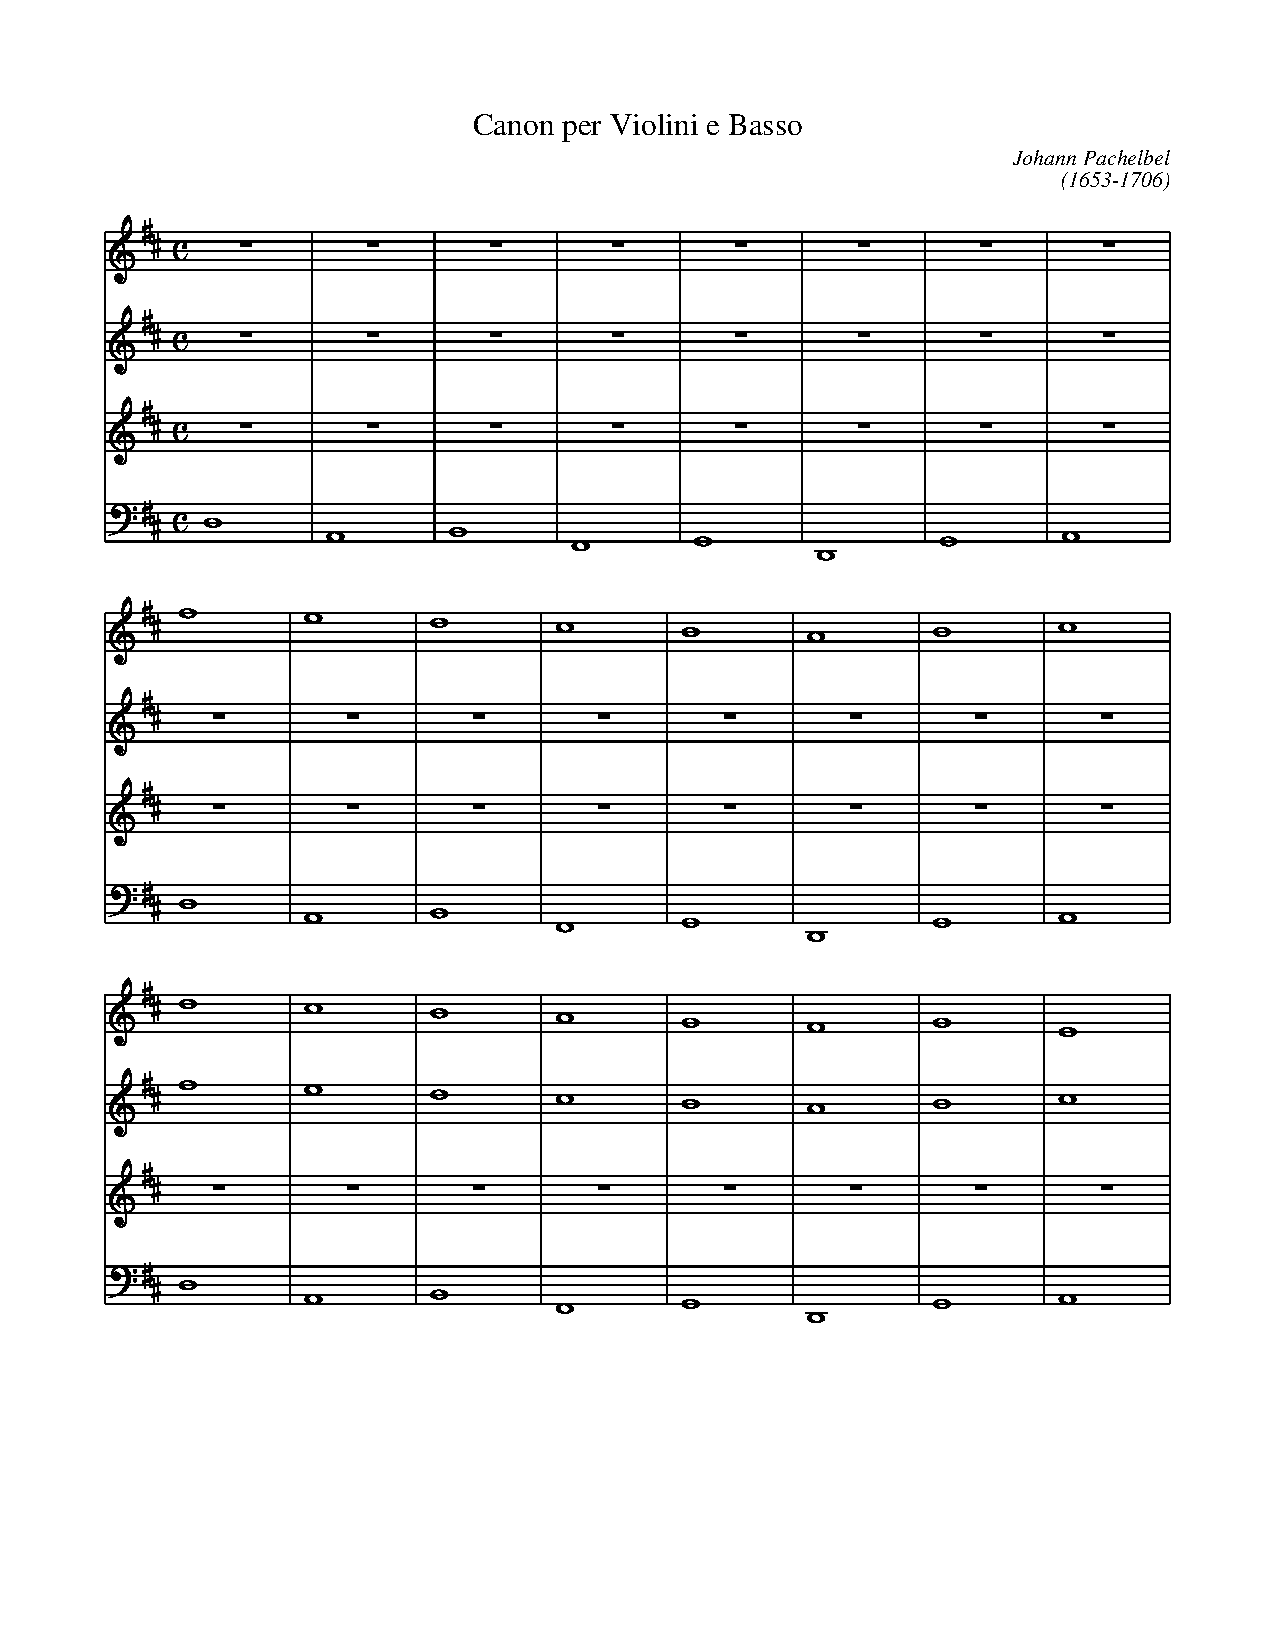
\includepdf[pages={1-7}]{img/pach_canon.pdf}
